%!TEX root = ../my_thesis.tex
\section[Correlation between $\Bz$ mass and decay time]{Correlation between \boldmath{$\Bz$} mass and decay time}
\label{app:invariantMassFit}

The small correlation between the $\Bz$ invariant mass and decay time is shown by comparing
the distribution of the decay time in bins of the invariant mass after applying the full
selection. This is done separately for signal and background. For the signal distribution
simulated data is used and the decay time is shown in six bins of the invariant mass.
(Fig.~\ref{fig:signalMassTime}).
\begin{figure}[b!]
  \begin{center}
   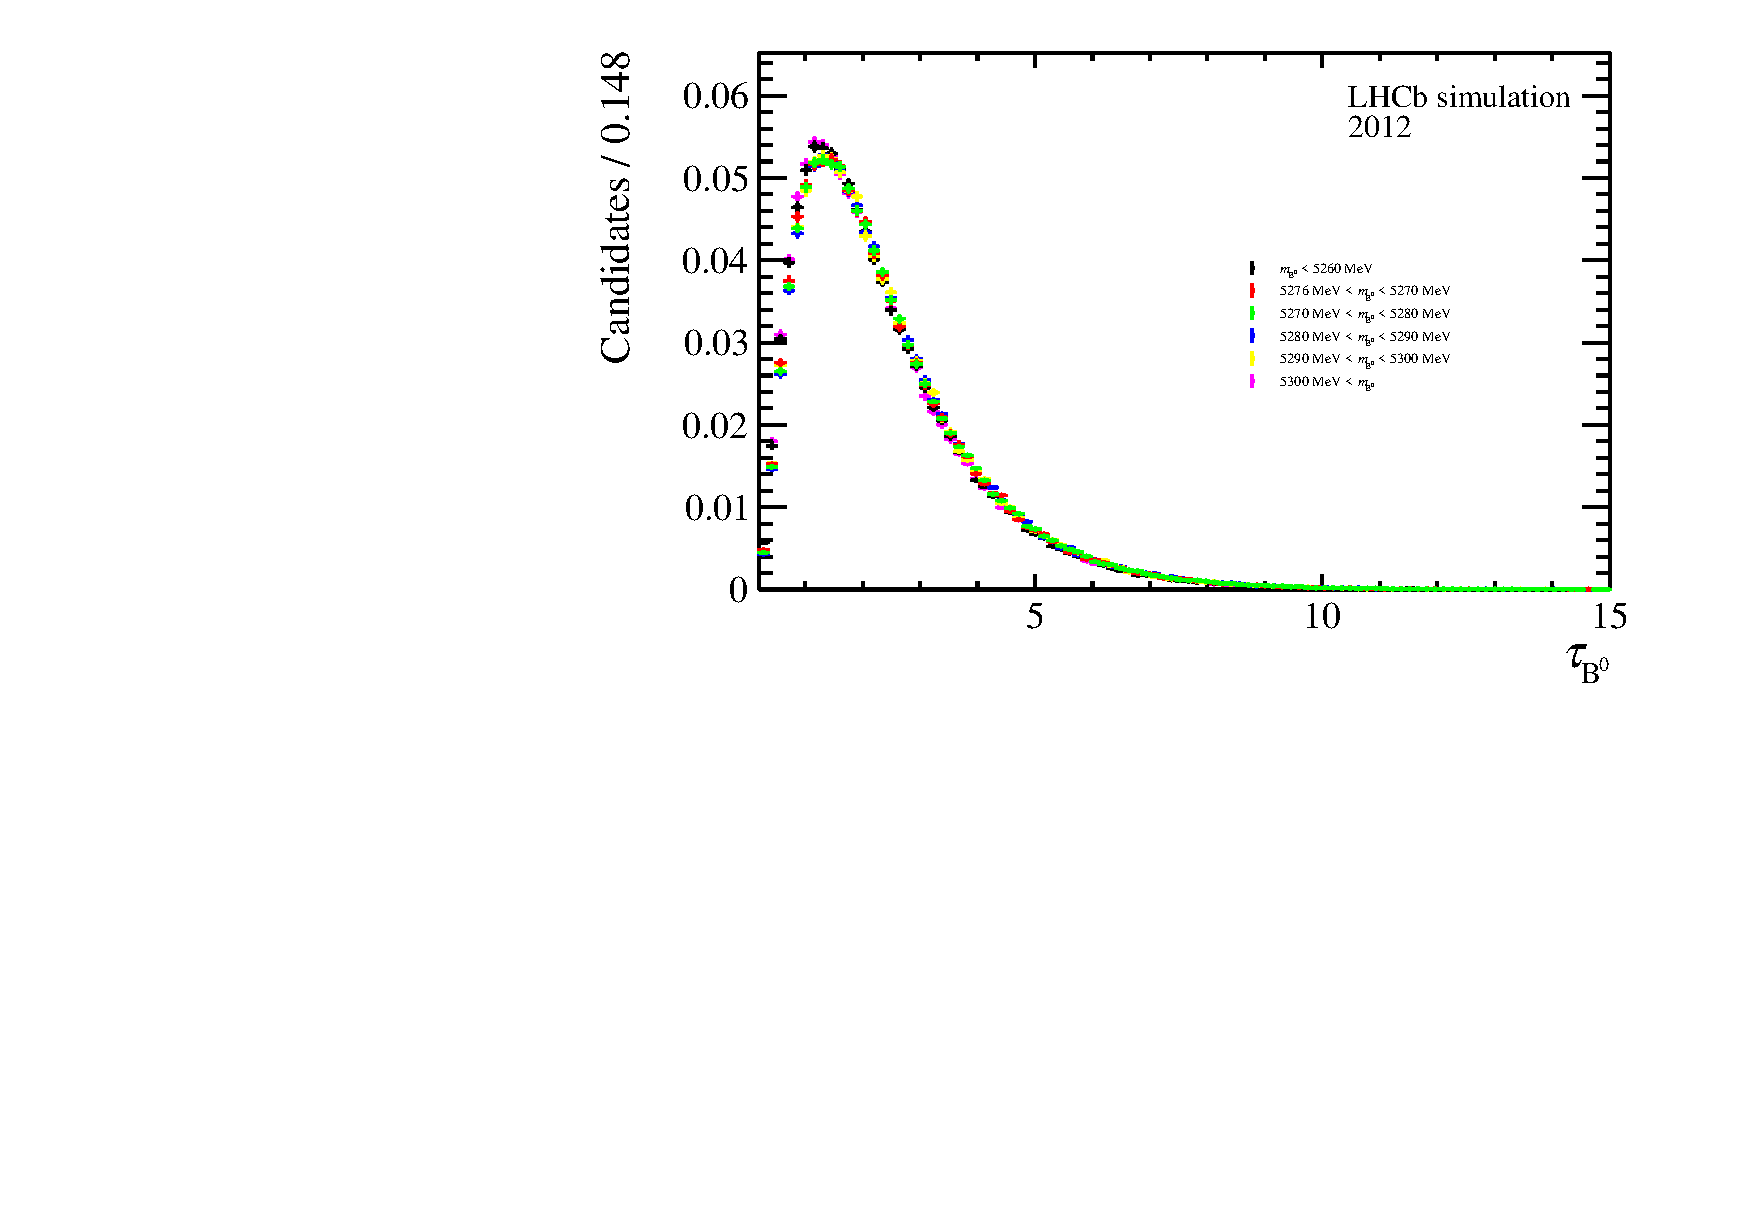
\includegraphics[width=0.5\textwidth]{AA-Appdx-massfit/figs/DecayTimeSignal.pdf}
  \end{center}
  \caption{Normalised MC signal decay time distributions in six bins of the reconstructed invariant mass.}
  \label{fig:signalMassTime}
\end{figure}
In order to account for the combinatorial background, the upper mass sideband is chosen as a
proxy. Figure~\ref{fig:bkgMassTime} shows the decay time in four bins of the invariant mass.
The physics background contribution in the signal region is considered to be small
enough, so that even a large correlation does not matter.
\begin{figure}[b!]
  \begin{center}
   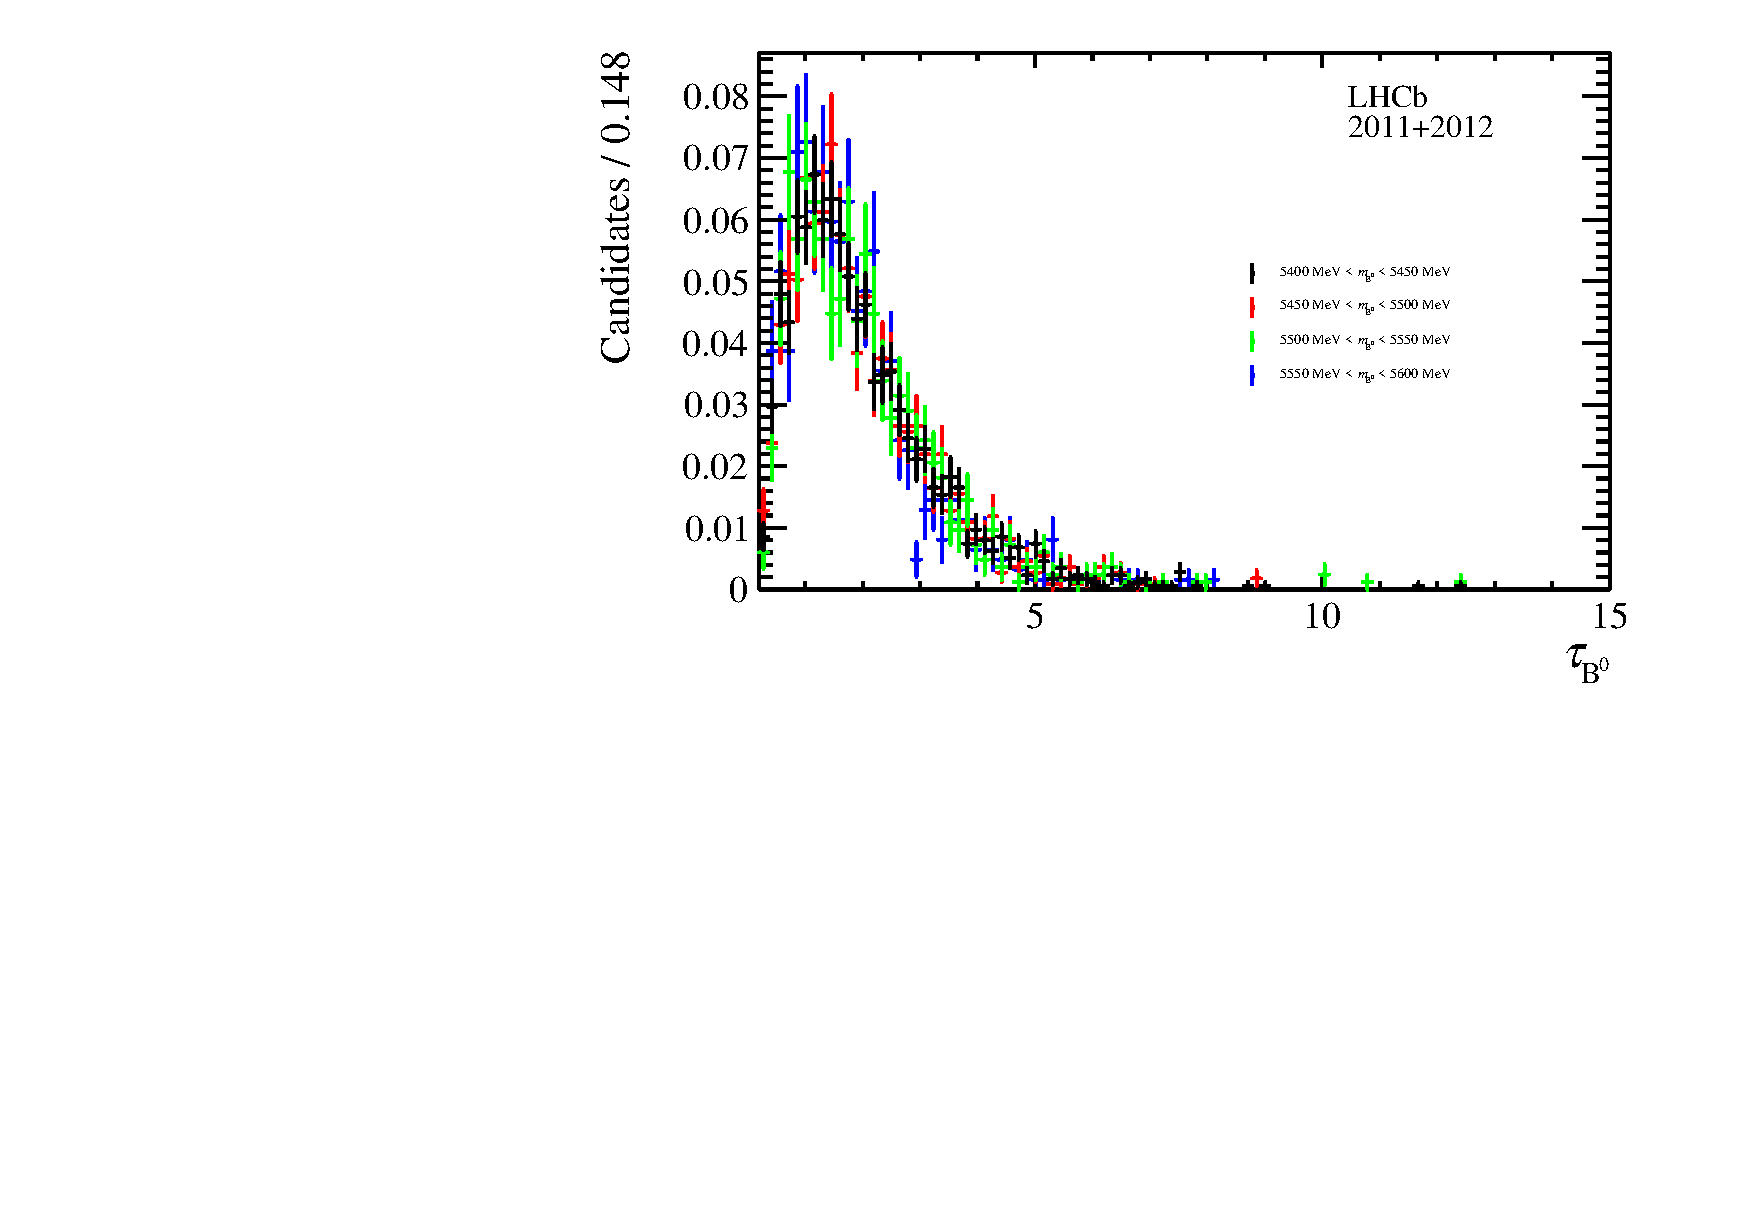
\includegraphics[width=0.5\textwidth]{AA-Appdx-massfit/figs/DecayTimeBkg.pdf}
  \end{center}
  \caption{Upper mass sideband decay time distribution in four bins of the
  invariant mass. The shapes are shown normalised.}
  \label{fig:bkgMassTime}
\end{figure}
Given the small differences for all distributions, the correlations between decay time and
invariant mass is assumed to be small enough to justify the use of the invariant mass in the \emph{sPlot}~\cite{sPlot} technique
for disentangling signal from background.
